\section{Presentation of research}
\label{presentation_of_research}
\subsection{Iterative Process}
% \subsubsection{First Sprint: Deep dive into Beckn}
% \label{first_sprint}
% % We could write something about the architecture and referring to DDD section, i think it would fit in well here.

% During the first sprint, our primary focus was to familiarize ourselves with the Beckn protocol, understanding its core concepts and functionality. To achieve this, we thoroughly explored the official documentation and watched the video series on their YouTube channel. Along the way, we discovered Beckn-ONIX, a promising tool that could help us quickly set up our Beckn network. All our insights and learnings from this sprint are detailed in Section \ref{beckn_protocol}.

% % With this knowledge in hand, we identified the necessary prerequisites for moving forward. We purchased a domain name from Simply.com and set up four servers on DigitalOcean, ensuring we were fully prepared for the next sprint. Confident in our understanding of the protocol and its workings, we felt ready to start building our Beckn-enabled network in the upcoming sprints.
\subsubsection{First Sprint: Deep dive into Beckn}
During the first sprint, our primary focus was to familiarize ourselves with the Beckn Protocol by understanding its core concepts and functionality. To achieve this, we thoroughly explored the official documentation and engaged with the video series available on the Beckn Foundation’s YouTube channel, particularly the Tech Overview playlist. This process deepened our understanding of the protocol’s architecture and its potential for decentralized applications. During this exploration, we discovered Beckn-ONIX, a promising tool designed to facilitate the rapid setup of a Beckn network. All our insights and learnings from this sprint are documented in Section~\ref{beckn_protocol}.

With a solid foundational understanding, we identified the necessary prerequisites for our network setup. We acquired a domain name from Simply.com and provisioned four servers on DigitalOcean to host the core components of the Beckn network. These preparations ensured that we were equipped for the subsequent sprint, confident in our ability to begin building the Beckn-enabled network.

The foundational knowledge from this sprint naturally aligned with Domain-Driven Design (DDD) principles, as discussed in Section~\ref{domain_driven_design}. DDD emphasizes the development of a Ubiquitous Language and the definition of a Bounded Context—concepts that seamlessly fit within the Beckn ecosystem. By engaging with Beckn’s resources, we established a shared vocabulary for components like Beckn Application Platforms (BAPs), Beckn Provider Platforms (BPPs), and the Beckn Gateway. This common language not only fostered effective communication within our team but also accurately reflected the domain-specific concepts necessary for our project.

Furthermore, we defined a Bounded Context for our envisioned decentralized food delivery network, adapting the protocol’s sector-agnostic framework to the specific domain of food ordering in Copenhagen. This DDD-inspired approach grounded our technical efforts in the domain’s needs, ensuring that our application of the Beckn Protocol was both technically robust and contextually relevant. These foundational steps set a clear and purposeful direction for the upcoming sprints.
\subsubsection{Second Sprint: Setting Up the Desired Platform}
\label{second_sprint}
The focus of the second sprint was to take what we had learned and attempt to deploy a working version of the Beckn-ONIX platform that could support a decentralized food delivery service. We followed the official setup guides and documentation to configure the four core components: Registry, Gateway, BAP, and BPP. 

While the guides provided some direction, many steps were either unclear or completely missing. Setting up reverse proxies, acquiring and configuring SSL certificates, and generating DNS records all required external research and trial-and-error. A good example of this was the reverse proxy setup. The setup guide provided example configs, which already contained SSL certificates, causing errors during Certbot execution. To work around this, we had to strip the default NGINX configuration of all HTTPS references and instead set it up with HTTP first. Once that worked, we were able to successfully generate the necessary SSL certificates and switch back to HTTPS.


Hardware limitations also caused issues during this sprint. Our initial deployment used virtual machines with 2~GB of memory, which led to Docker containers silently crashing and entering a reboot loop. Even upgrading to 4~GB did not resolve the issue completely. It was only after switching to 8~GB instances that the containers became stable. There was no documentation regarding hardware requirements, which meant we had to find the fitting hardware specs based on trial and error, which caused this process more frustrating and time-consuming than it needed to be.

Below is a graph showing the CPU and memory usage of the machines while running the Beckn-ONIX install script. The BAP and BPP virtual machines are almost identical to each other in terms of usage, as well as the registry and gateway are. \newpage

\begin{figure}[h!]
    \centering
    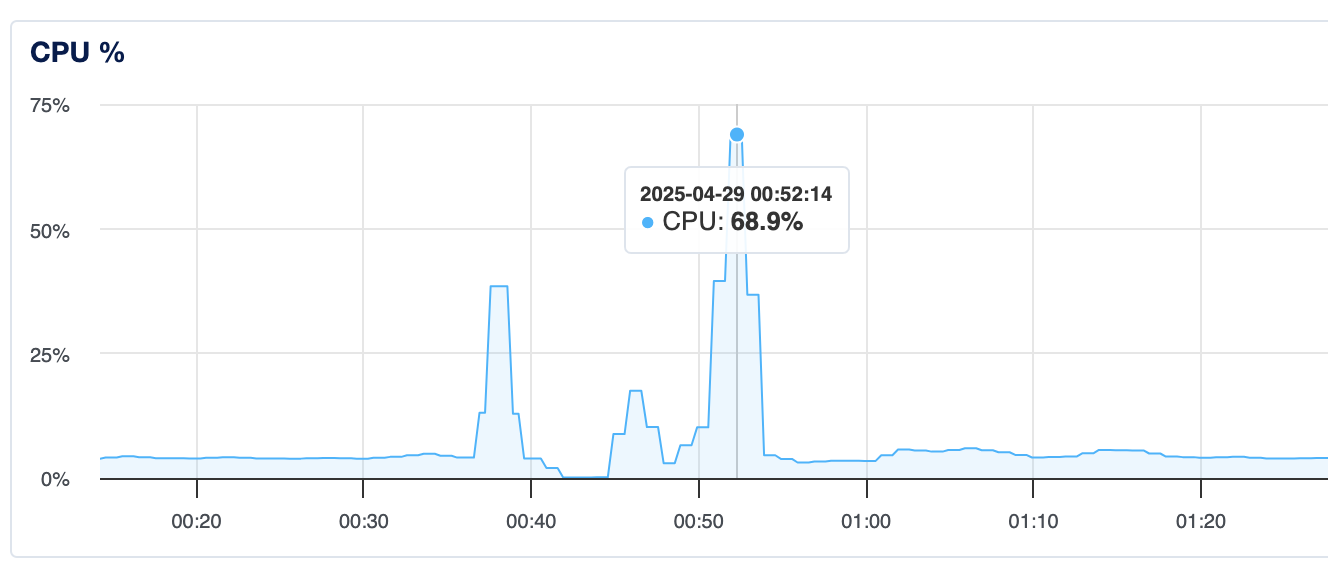
\includegraphics[width=0.49\textwidth]{Images/bap_cpu.png}%
    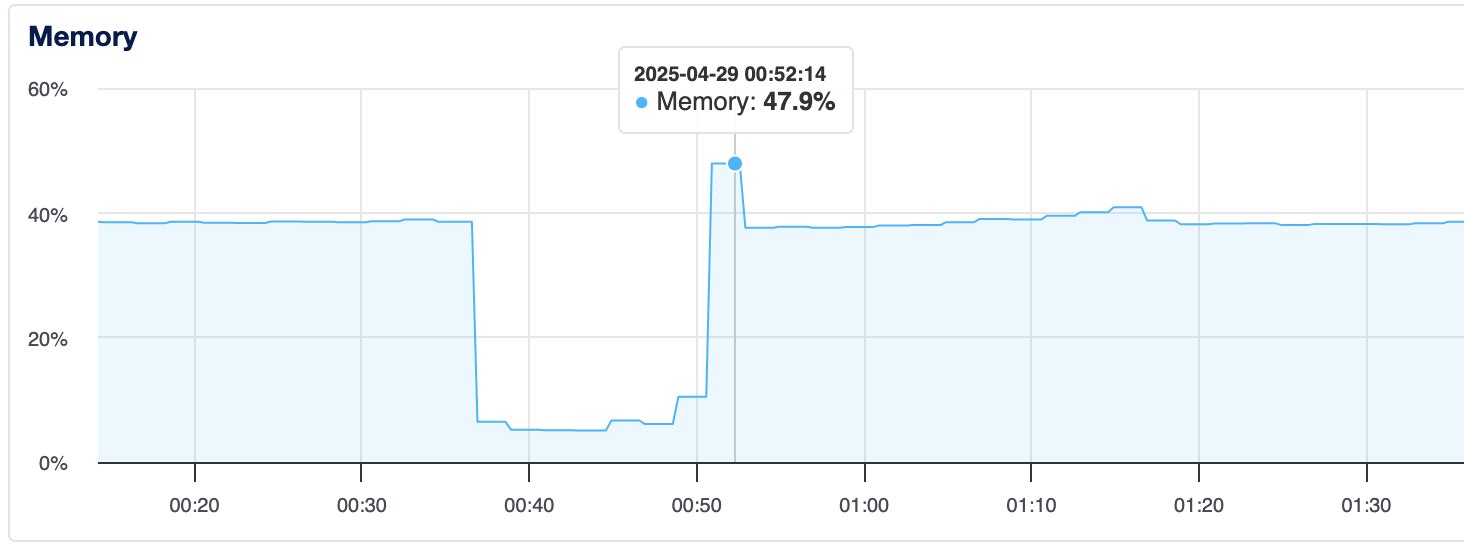
\includegraphics[width=0.49\textwidth]{Images/bap_ram.png}
    \caption{CPU and Memory usage of the BAP virtual machine, while running Beckn-ONIX install}
    \label{fig:bap_usage}
\end{figure}
\begin{figure}[h!]
    \centering
    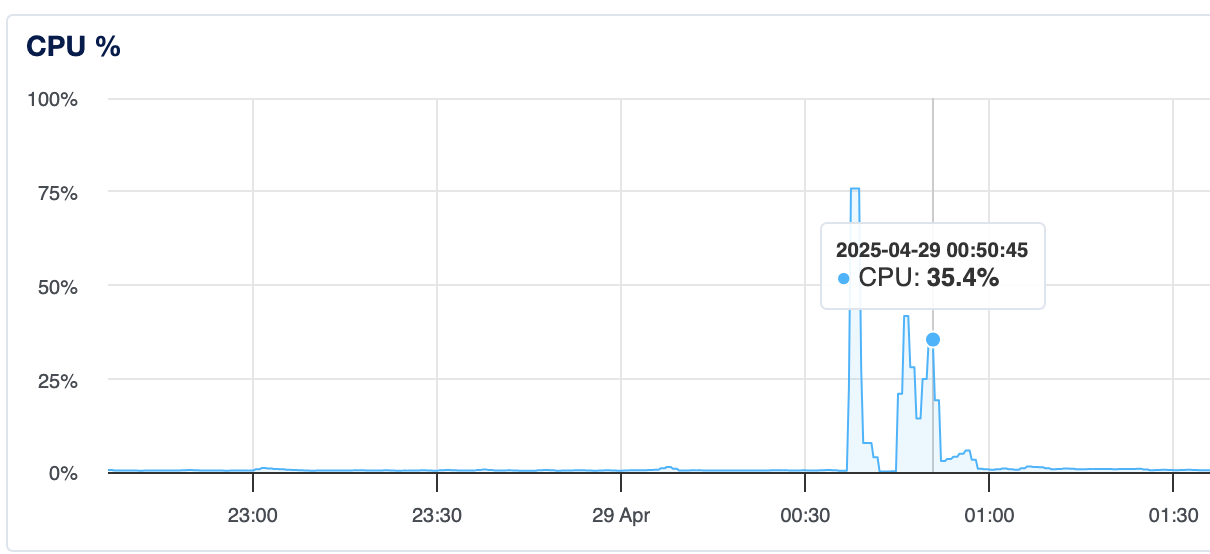
\includegraphics[width=0.49\textwidth]{Images/registry_cpu.png}%
    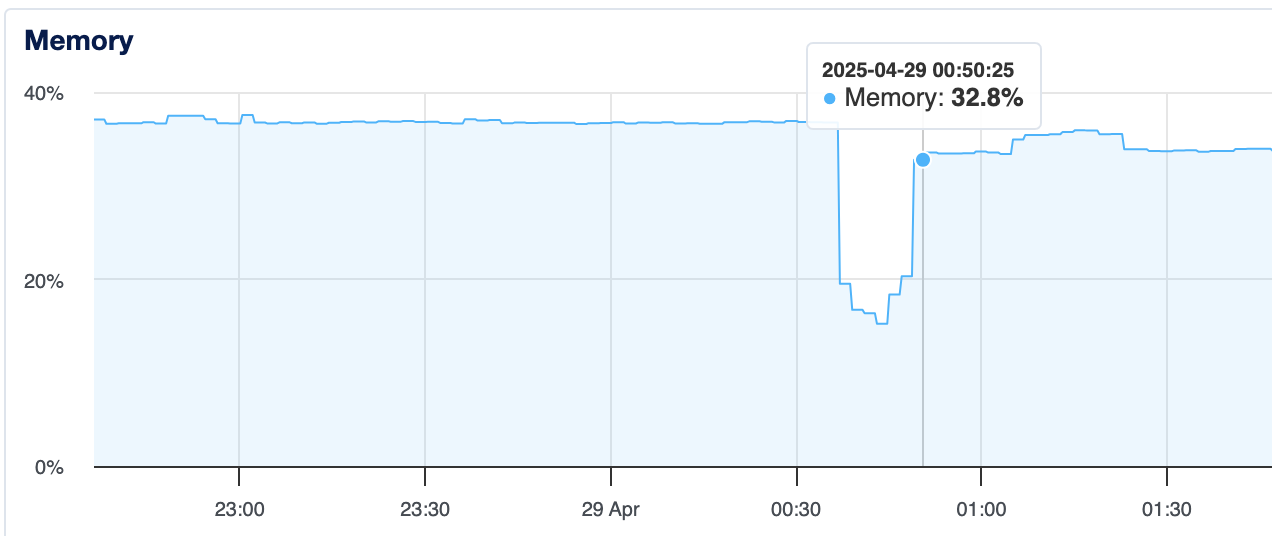
\includegraphics[width=0.49\textwidth]{Images/registry_ram.png}
    \caption{CPU and Memory usage of the registry virtual machine, while running Beckn-ONIX install}
    \label{fig:registry_usage}
\end{figure}


Setting up DNS configurations went relatively smoothly. We bought a domain through Simply.com and used their interface to configure the necessary subdomains such as \texttt{bap.domain.dk}, \texttt{bpp.domain.dk}, \texttt{registry.domain.dk}, and so on. This part was quite intuitive, and once the subdomains pointed to the correct servers, it aligned well with the expected Beckn-ONIX structure. 

A major challenge during this sprint was setting up the domain-specific webhook. The CLI documentation referenced a sample webhook, but it was not clearly documented how it fit into the system. We eventually figured out that each BPP server must provide a webhook endpoint to handle callbacks from the Gateway. We built a custom Node.js webhook and wired it up manually so the BPP could respond to incoming requests.

Despite the hurdles, by the end of this sprint we had a functioning network. We were able to send requests through Postman to our BAP server, which forwarded them to the Gateway, and ultimately received responses back from the BPP. The BPP successfully interacted with our custom webhook to generate the expected responses.

The following sequence diagram illustrates the flow of a search request initiated from Postman within the Beckn Network. It outlines the interactions between various components, including Postman, Bap Client, BAP, Gateway, Registry, BPP, BPP Client, and Webhook. The diagram reflects both the expected results and the actual outcomes observed by analyzing the logs from different domain endpoints.\newpage

\begin{figure}[h!]
    \centering
    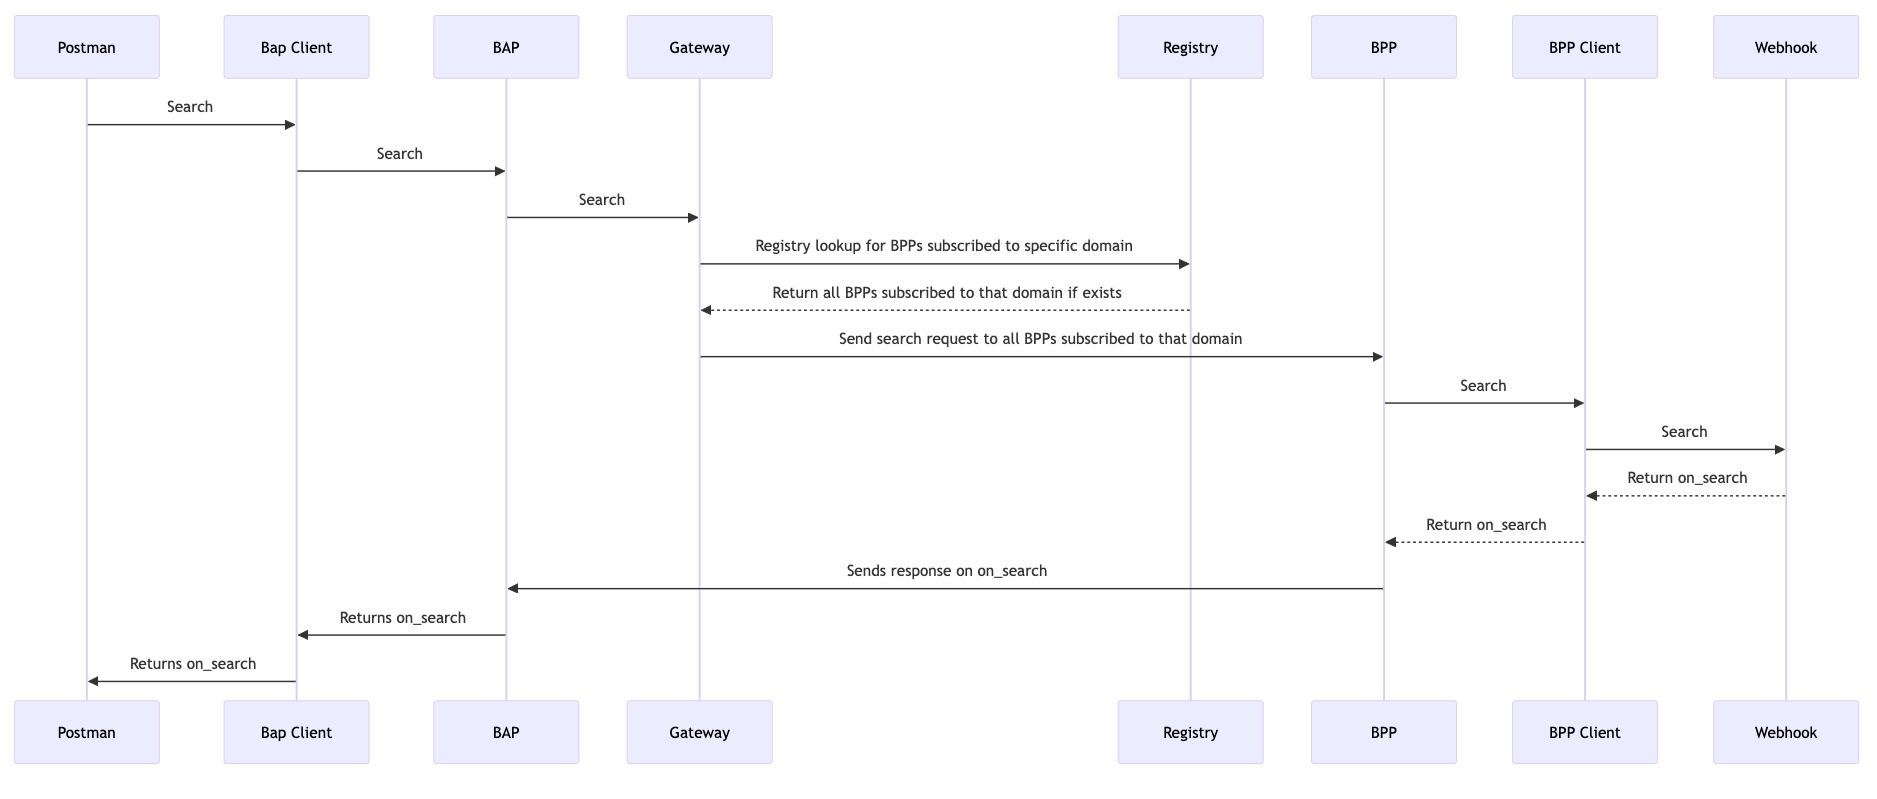
\includegraphics[width=1.0\textwidth]{Images/search_sequence.png}
    \caption{Sequence diagram of a search request from Postman to the bap-client}
    \label{fig:enter-label}
\end{figure}

However, it had been such a time consuming and frustrating journey, that we felt that a better contribution would be to integrate all of our findings into a script that automatically handles the setup process, saving all future developers a lot of time, allowing them spend their resources on innovative networks rather than setup-struggles. 
\subsubsection{Third Sprint: Creating the Orchestrator Script}
\label{third_sprint}
In our third sprint, we combined every insight from the previous two iterations into a single “orchestrator” shell script that aims to fullfil Beckn-ONIX’s promise of a near plug-and-play deployment. Having found solutions to all of the issues like reverse-proxy adjustments, SSL provisioning via Certbot, webhook setup, and hardware requirements; we tried to combine all our findings into a single automation script so that future developers could set up a complete Beckn network in minutes rather than days.

We chose to remain consistent with the Beckn community current scripting conventions and rely on plain Bash scripts orchestrated over SSH. This choice ensures maximum portability: as long as a server allows SSH, our orchestrator script will provision the registry, gateway, BAP, BPP and a test webhook endpoint without the user ever touching NGINX configs.

We built the script around three Infrastructure as Code principles modularity, parameterization and external configuration, which is described in Section~\ref{modularization} Section~\ref{parameterization_external_config}

Because we played the dual role of developer and user throughout Sprints 1 and 2, our workflow organically followed a User-Centered Design cycle—understand context, specify requirements, design a solution, and evaluate against real pain points \citep{norman_1986}.

Reflecting on the finished product, we recognize that there are still further improvements to be made: making each step idempotent so that re-runs simply skip already completed tasks, assess error handling with clear exit codes and hints on how to fix it, and improving logging so that users see meaningful progress rather than undifferentiated shell output. By automating Beckn-ONIX setup in this orchestrator, we not only save valuable development hours but also pave the way for others to innovate on top of Beckn, rather than struggle with the setup.

\subsection{Product}
\label{product}
For the final product, an Infrastructure as Code tool has been created, complying with the style of the Beckn-ONIX community, by utilizing shell scripts to minimize dependencies and new tools, as well as good code principles both for software design, software architecture, DevOps principles and design principles as described throughout the project report (refer to relevant sections). Furthermore a thorough README has been made to guide users of how to run the script, as well as filling in the missing gaps of documentation we felt was lacking from the official Beckn-ONIX setup guide - the README can be found in appendix \ref{readme_appendix}. 

The tool is aiming to ease the setup of a full production like environment, that is able to fulfill a transaction running on the Beckn network. This section will go into details about the final product, how it works and what it does.

\subsubsection{Orchestrator script}
\label{product_orchestrator}
The orchestrator script is responsible for executing all child scripts in the correct sequence, ensuring that each task is run on the appropriate server and under the right conditions. Each child script is designed with a single, clearly defined purpose and stripped of excess logic to remain simple, maintainable, and easy to modify. While the orchestrator handles the flow and environment setup, the child scripts remain focused solely on their specific configuration or deployment task.

Tasks that are not dependent on being completed sequentially across all servers are executed in parallel to optimize time efficiency. This parallel execution is also managed by the orchestrator, which ensures that asynchronous tasks are coordinated properly, without compromising the stability of the overall process. The figure below illustrates the execution flow of the orchestrator script and all of the child script it is handling. The full script can be found in appendix \ref{orchestrator_appendix}.\newpage

\begin{figure}[h!]
    \centering
    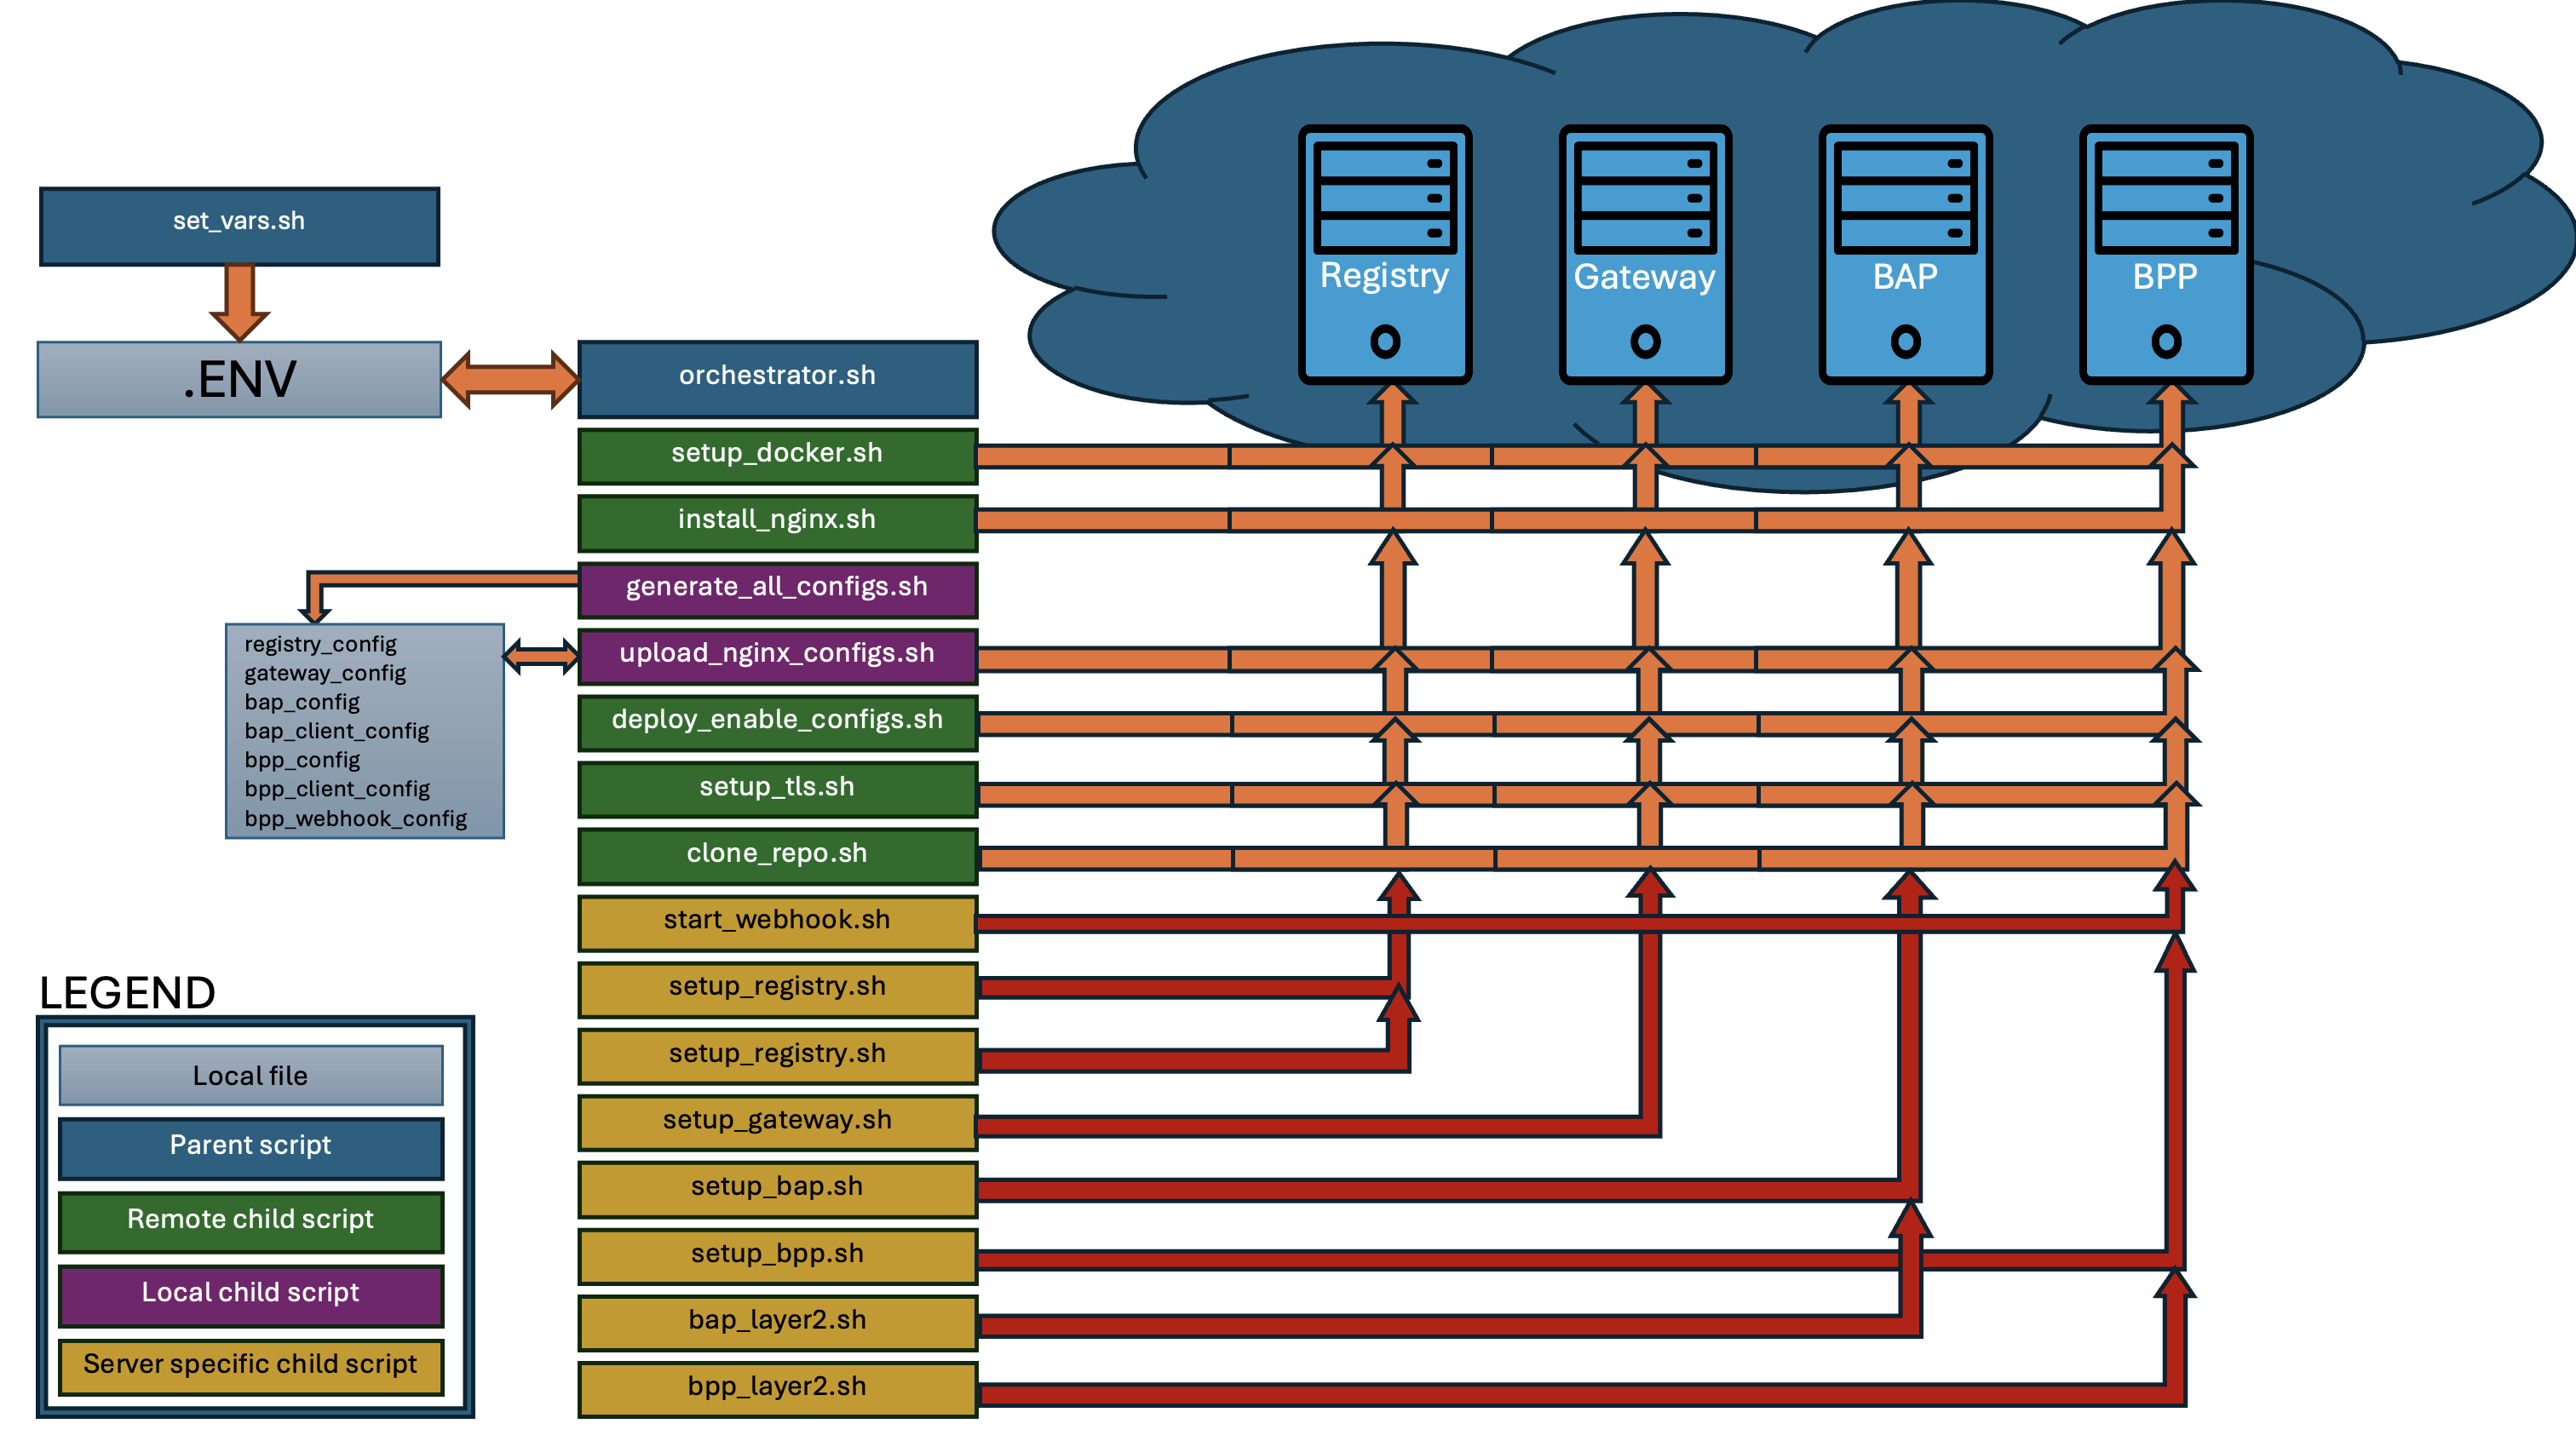
\includegraphics[width=1\textwidth]{Images/orchestrator_architecture.png}
    \caption{Orchestrator script architecture}
    \label{fig:Orchestrator_architecture}
\end{figure}

There are three types of execution modes available for child scripts: \texttt{remote}, \texttt{local}, and \texttt{server}. Each script is tagged accordingly, and the orchestrator uses a case statement to determine how it should be executed:

\begin{minted}[fontsize=\small, bgcolor=gray!5, frame=lines, linenos]{bash}
for task in "${TASKS[@]}"; do
    IFS=':' read -r script type server <<< "$task"
    case "$type" in
        remote)
            run_script_on_all "$script"
            ;;
        local)
            run_local_script "$script"
            ;;
        server)
            run_script_on_server "$script" "$server"
            ;;
        *)
            echo "Unknown task type: $type for script: $script"
            exit 1
            ;;
    esac
done
\end{minted}

The child-scripts with the \texttt{remote} label, will be executed by the \texttt{run\_script\_on\_all()} function that has been designed to handle remote execution in parallel. The function takes the name of a script and executes it concurrently on all target servers defined in the configuration array. It establishes SSH connections to each server, exporting environment variables dynamically by parsing a shared \texttt{.env} file, and injects them into the remote execution context. Each script execution is initiated in the background using Bash’s asynchronous process handling \texttt{(\&)}, enabling parallelism. The function then tracks the completion status of all remote executions using process IDs and provides aggregated success or failure reporting.

Child scripts labeled with the \texttt{local} tag are executed using the \texttt{run\_local\_script()} function. This function is responsible for running the specified script locally on the host machine where the orchestration is initiated. It takes the script name as input, resolves its path relative to the orchestration directory, and executes it using Bash. The function provides basic success or failure reporting by evaluating the script's exit status. If the script completes successfully, a confirmation message is logged; otherwise, an error message is shown and the orchestration process terminates to prevent further execution. This ensures that local setup steps are validated and enforced before continuing with distributed deployment steps.

Scripts labeled with the \texttt{server} tag are executed using the \texttt{run\_script\_on\_server()} function, which targets a single, explicitly specified server (e.g. registry, gateway, BAP). This function accepts both the script name and the destination server address as arguments. Similar to the parallel remote execution method, it dynamically constructs environment variables by parsing a shared .env file and injects them into the remote execution context. It then establishes an SSH connection to the given server and runs the script via a remote shell. Unlike the remote variant, this function runs sequentially and is intended for cases where a task must be performed on a specific server instance rather than all servers. It includes success and failure handling to enforce reliability during critical one-to-one deployment steps. 

\subsubsection{Modularity and Single Responsibility}
\label{modularity_single_responsibility}
The orchestrator script is designed with modularity in mind (section~\ref{modularization}), executing 15 distinct tasks defined in a TASKS array, each handled by a dedicated child script with a single responsibility. These tasks are categorized as remote (e.g. \texttt{setup\_docker.sh}, run in parallel on all servers), local (e.g., generate\_all\_configs.sh, run on the user's machine), or server-specific (e.g., \texttt{setup\_registry.sh}, is run sequentially on the designated servers). This structure ensures flexibility and maintanability, allowing users to modify or extend individual scripts without altering the orchestrator. Also it gives full transparency on where each child script is executed from the orchestrator. 

\subsubsection{NGINX Configuration} \label{nginx_configuration}
The script automates the generation of seven NGINX configuration files for the registry, gateway, BAP, BAP-client, BPP, BPP-client and webhook, using the \texttt{DOMAIN\_NAME} and subdomains from the \texttt{.env} file. All the configuration files are mainly generated from the example configurations provided by Beckn-ONIX \citep{becknNginxConfig}, but with slight modifications. The \texttt{generate\_all\_configs.sh} script (which calls component-specific scripts like \texttt{generate\_bpp\_config.sh}) creates these configs, and \texttt{deploy\_enable\_configs.sh} automates symbolic links to enable them. Unlike the manual process, which required hours of configuration and caused Certbot failures due to premature SSL references in Beckn-ONIX example configurations, the script ensures error-free setups by generating HTTP-only configurations compatible with Certbot.

This automation reduced the complexity a lot, as well as sped up the deployment time. Compared to having to ssh into servers and create configuration files, enable them, request certificates 7 times over, this script feels almost instantaneous.

\subsubsection{.env File and Parameterization}
\label{env_config}
The \texttt{.env} file enables parameterization, allowing users to deploy a Beckn network for any domain by specifying key variables like \texttt{DOMAIN\_NAME} and server IP's with the help of the \texttt{set\_vars.sh} script (section~\ref{parameterization_external_config}). Additional variables such as subdomains (e.g., onix-registry), are generated automatically with the names we have used, to ease out the process of setting them all up at once. In case the subdomains are not aligned with the ones we have used, it still creates a good template that is easy to change from there and with the all of the necessary variables in place. 
This parameterization enhances the script's flexibility, while it is centralized and separated from logic it allows for other developers to easily adapt into it, even if they where to have other ideas for naming conventions.

\subsubsection{Open-Source Contribution}
\label{open_source_contribution}
Our orchestrator script is an open-source contribution to the Beckn ecosystem, publicly available at \url{https://github.com/Bachelors-Project-frlr-raln/beckn-IaC/tree/v1.0.2}. This aligns with the collaborative ethos of the GNU Manifesto, which advocates for software as a shared resource to empower users \citep{stallman1985gnu}. By providing a detailed README and modular, parameterized scripts, we lower technical barriers, enabling developers—especially small teams or newcomers—to deploy Beckn networks efficiently. This open-source approach fosters innovation, allowing the community to build on our work, adapt it to diverse domains, and realize applications like the decentralized food delivery network we initially envisioned. Our contribution supports Beckn’s mission of inclusive digital marketplaces, as discussed in Section~\ref{IaC_discussion}.

\subsection{Evaluation and Verification}
\subsubsection{User Testing}
To assess the automation script’s effectiveness and its implementation guide, we conducted structured user testing. The goal was to evaluate usability and accessibility for developers with skills similar to ours at the project’s start, including those with limited experience. We also tested compatibility across Windows with Windows Subsystem for Linux (WSL) and Linux, ensuring functionality despite differences from our macOS development environment.

Three sixth-semester BSc students from the IT University of Copenhagen participated. Two had taken the same DevOps course as us, while the third had not, allowing us to gauge accessibility for users with minimal background. Two used Windows with WSL, and one used Debian Linux.

To focus testing on the script and Beckn-specific deployment, we provided a preconfigured environment with four DigitalOcean droplets meeting minimum server requirements, pre-set DNS records, and SSH access. Participants received server IPs and the domain name, which they input into the \texttt{set\_vars.sh} script. This ensured the evaluation targeted the script’s performance, not server or DNS setup skills. Participants deployed a Beckn production network using only the README documentation.

We used the think-aloud protocol \citep{nielsen_1993}, effective for identifying usability issues in software tools. Participants verbalized their decisions during deployment, while we observed actions, monitored screens, and noted issues or errors. This qualitative approach provided insights into the script’s ease of use, documentation clarity, and any challenges.

\subsubsection{Results and Analysis}
All participants successfully deployed a Beckn production network and completed a mock transaction via Postman in under 15 minutes, despite no prior Beckn knowledge. This efficiency, including dependency installation and README review, confirms the script’s usability and accessibility. No major errors occurred across Windows WSL and Linux, validating cross-platform reliability.

Minor README feedback included adding quotes around a `+' symbol and labeling the gateway IP for clarity. These actionable suggestions were incorporated, aligning with continuous improvement principles (Section~\ref{CSE_improvements}). The success of participants with varying expertise, including one without DevOps experience, highlights the script’s accessibility for non-expert developers. These findings address the research question, demonstrating that the script maximizes usability and minimizes deployment time, lowering barriers for the Beckn community, especially for small teams or new developers.

\subsubsection{Technical Contributions and Impact} \label{tech_contribution_and_impact}
The orchestrator script streamlines Beckn production network deployment, reducing time, ensuring stability, and enhancing automation, as grounded in Infrastructure as Code (IaC) principles (Section~\ref{sectionIaC}) and DevOps practices (Section~\ref{devops}).

\begin{itemize}
    \item \textbf{Time Efficiency}: The script reduces deployment time by 99\%, from days to $\sim$15 minutes, compared to our initial manual setup. Parallel execution of tasks (e.g., Docker installation, NGINX configuration) across four servers (registry, gateway, BAP, BPP) cuts combined duration by 75\% (see Figure~\ref{fig:Orchestrator_architecture}). Automated generation of seven NGINX configurations and TLS certificate acquisition via Certbot eliminates error-prone manual steps, fulfilling Beckn-ONIX’s rapid-deployment promise.
    \item \textbf{Stability and Performance}: The script prevents hardware-related issues, such as silent Docker crashes on under-provisioned machines, by codifying requirements: 8GB RAM and 2 Intel vCPUs for BAP/BPP servers, and 2GB RAM with 1 vCPU for registry/gateway (see Figures~\ref{fig:bap_usage} \&~\ref{fig:registry_usage}). These specifications, derived from Sprint 2 trial-and-error, ensure stability during setup and under load.
    \item \textbf{Automation Benefits}: By automating 15 tasks, including component setup and configuration, the script reduces manual steps by $\sim$90\%. Its modular, parameterized design enhances maintainability and flexibility, allowing deployment across domains via the \texttt{.env} file. This codifies setup knowledge, serving as executable documentation.
\end{itemize}

These contributions enable developers to focus on innovative Beckn applications, like the envisioned food delivery network, rather than setup challenges. The script supports the Beckn community’s open-source ethos and DevOps practices, such as reproducible environments, directly addressing the research question by optimizing setup usability and efficiency.